% Tormenta v2: full project report (nowcaster + 7-day forecaster + locked model).
% Compile on Overleaf (pdfLaTeX). Upload the whole docs/report/v2/ folder; figures are in figs/.
% Test-period numbers come from the one-time test of the locked model (DECISIONS D-76/D-77).
\documentclass[11pt,a4paper]{article}
\usepackage[a4paper,margin=2cm]{geometry}
\usepackage[T1]{fontenc}
\usepackage{lmodern}
\usepackage{microtype}
\usepackage{graphicx}
\usepackage{booktabs}
\usepackage{tabularx}
\usepackage{longtable}
\usepackage{amsmath}
\usepackage{caption}
\usepackage{subcaption}
\usepackage{enumitem}
\usepackage{xcolor}
\usepackage{tikz}
\usetikzlibrary{arrows.meta,positioning,fit,backgrounds}
\usepackage[section]{placeins}
\usepackage[colorlinks=true,linkcolor=black,citecolor=black,urlcolor=blue!50!black]{hyperref}
\graphicspath{{figs/}}
\captionsetup{font=small,labelfont=bf,skip=3pt}
\setlist{nosep,leftmargin=*}
\setlength{\textfloatsep}{10pt plus 2pt minus 2pt}
\renewcommand{\arraystretch}{1.08}
\newcommand{\code}[1]{\texttt{\small #1}}
\newcommand{\tbd}[1]{\textcolor{red}{\textbf{[#1]}}}
\newcolumntype{Y}{>{\raggedright\arraybackslash}X}

\title{\vspace{-1.2em}\textbf{Tormenta v2: Nowcasting and 7-Day Forecasting of Geomagnetic Activity\\
from Ground Indices, Solar Wind and Solar EUV Images}\vspace{-0.4em}}
\author{Syeda Aliza Ayaz (CT-24219) \quad Husn ur Rehman (CT-24070)\\[1pt]
\small CT-378 Machine Learning, NED University of Engineering \& Technology, Fall 2026\\[1pt]
\small Code: \url{https://github.com/Syeda-Aliza-Ayaz/Tormenta} \quad Live app: \url{https://tormenta.streamlit.app/}}
\date{\vspace{-1.6em}}

\begin{document}
\maketitle

\begin{abstract}
\noindent Tormenta is a two-part geomagnetic activity system. The \textbf{nowcaster} estimates the planetary Kp
index for the current hour from solar-wind data measured about an hour upstream of Earth (66 causal features,
HistGradientBoosting, test RMSE 0.573 Kp, $R^2$ 0.808, calibrated 80\% interval). The \textbf{forecaster} issues
daily Ap and daily maximum Kp for lead days 1--7, with storm-day probabilities. It started from past indices only
(29 features; test skill +0.100 against the 27-day average, level with NOAA's official forecast on days 1--3). A
nine-year validation harness with adoption rules fixed before each run then selected two input groups: daily solar
wind with its 27-day echo (16 features) and coronal-hole measurements from one SDO/AIA 193\,\AA{} image per day
(7 features). On 2013--2019 this raised Ap skill from 0.131 to 0.160 and lead-day 2--4 skill from 0.110 to 0.155,
winning in 7 of 7 years. Leakage controls (a one-day image delay and a shuffled-date placebo) confirm that the gain
comes from the images. The resulting model, \textbf{HistGB-SW-CH}, was locked and committed before the test period
(2020-01 to 2026-06) was read, then scored once. On 2{,}373 test days it raised skill from 0.100 to 0.122 (95\%
block-bootstrap interval of the gain $+0.007$ to $+0.050$) and mean storm Heidke on days 1--3 from 0.25 to 0.31, with
fewer false alarms. It is level with NOAA's official forecast (no significant difference on days 1--3). Every forecast is logged before its
day, scored against GFZ Potsdam, and compared with NOAA SWPC.
\end{abstract}

\tableofcontents
\clearpage

%----------------------------------------------------------------------------------------------------------------
\section{Problem and motivation}
Geomagnetic storms disturb power grids, satellite operations, GNSS positioning and HF radio. Their strength is
summarised by the planetary \emph{Kp} index (``planetarische Kennziffer'', 0--9 in thirds, one value per 3-hour
block) and its linear equivalent \emph{ap} (0--400). The daily \emph{Ap} is the mean of the day's eight ap values
\cite{matzka2021}. A \emph{storm day} in this project is a day whose maximum Kp is at least 5$-$ (4.67), NOAA's G1
level.

Two questions are useful to an operator, and they need different information:
\begin{enumerate}
\item \textbf{What is Kp now?} The solar wind measured at L1, 1.5 million km upstream, arrives about an hour later,
so the current hour can be estimated before ground magnetometers report (\emph{nowcast}).
\item \textbf{What will Ap and Kp be on each of the next 7 days?} Nobody measures the solar wind days ahead. The
information that remains is past activity, the 27-day solar rotation, the solar cycle, the season, and what can be
seen on the Sun's Earth-facing disk (\emph{forecast}).
\end{enumerate}
Version 1 of this project (the course report) covered the nowcaster. Version 2 adds the forecaster, its
improvements, and the locked final model, and compares it with NOAA's official forecasts \cite{swpc}.

%----------------------------------------------------------------------------------------------------------------
\section{Datasets}
All data are public. NOAA forecasts are a \emph{benchmark only} and are never used as inputs (D-06), so any skill
we report is our own.

\begin{table}[htbp]\centering\small
\caption{Datasets. ``Use'' shows where each enters the system; dates are the spans used.}\label{tab:data}
\begin{tabularx}{\textwidth}{@{}p{3.1cm}Yp{3.3cm}p{2.9cm}@{}}\toprule
Dataset & Content & Span & Use\\\midrule
GFZ Potsdam Kp/Ap \cite{gfzkp} & 3-hourly Kp, ap; daily Ap; observed F10.7; definitive flag & 1932 $\to$ (daily file) & forecaster inputs; every label and score\\
NASA OMNI2 hourly \cite{king2005} & $|B|$, $B_x$, $B_y$, $B_z$ (GSM), speed, density, temperature; shifted to the bow shock & 1998 $\to$ 2026-11 (SPDF yearly files) & nowcaster training; forecaster solar-wind training\\
NOAA SWPC real-time \cite{swpc} & propagated 1-min solar wind (7 days), F10.7, estimated Kp & live & nowcaster input; live solar-wind archive\\
SDO/AIA 193\,\AA{} \cite{lemen2012,pesnell2012} & one 1024$\times$1024 level-1.5 image per day at 00:00 UTC (JSOC synoptic archive; near-real-time folder live) & 2010-05-13 $\to$ & coronal-hole features\\
NOAA 3-day forecast, RSGA \cite{swpc} & Ap forecasts days 1--3; storm probabilities & 2017 $\to$ & benchmark only\\
NASA DONKI CME catalogue & CME speed, width, arrival & 2014 $\to$ & experiment D-67 (rejected)\\
NOAA event reports & flares, radio bursts, protons & 1996 $\to$ & experiment D-74 (rejected)\\\bottomrule
\end{tabularx}
\end{table}

\paragraph{Sizes.} The nowcaster uses 245{,}688 hourly rows (about 81{,}900 independent 3-hour labels). The
forecaster uses 34{,}653 daily rows (1932-01-01 to 2026-11-15), trained from 1947-06-01, the first day on which the
81-day F10.7 mean exists (D-19). The image set holds 3{,}489 files for 2010--2019 (3{,}467 usable days after the
quality filter) and 2{,}367 for the test period (2{,}360 usable days of 2{,}373).

\paragraph{Splits (time-ordered, never shuffled).}
\begin{itemize}
\item Nowcaster: train 1998--2016, validation 2017--2019, test 2020--Jan 2026.
\item Forecaster: train 1947-06--2016, validation 2017--2019 (later the yearly harness 2011--2019, \S\ref{sec:eval}),
test 2020-01-01 to 2026-06-30 (2{,}379 days, 325 storm days). The test period was scored once for the v2.0 models
(D-52/D-62) and once for the locked model (D-77).
\end{itemize}

%----------------------------------------------------------------------------------------------------------------
\section{Data pipeline and preprocessing}\label{sec:pipeline}
Figure~\ref{fig:pipeline} traces each data source from download to model input. Three rules shape it:
\begin{itemize}
\item \textbf{No preprocessing step is fitted on data the model will be scored on.} Cleaning steps have no fitted
parameters, and the only fitted steps (imputation and scaling) sit inside scikit-learn pipelines fitted on training
rows only \cite{pedregosa2011}.
\item \textbf{Gaps stay gaps.} Missing hours and days are never filled from the future. HistGB routes missing values
natively, so only the linear, KNN and SVR nowcasters need imputation.
\item \textbf{Causality is tested.} Automated tests delete or alter every value after the issue time and check that
the features do not change.
\end{itemize}

\begin{figure}[htbp]\centering
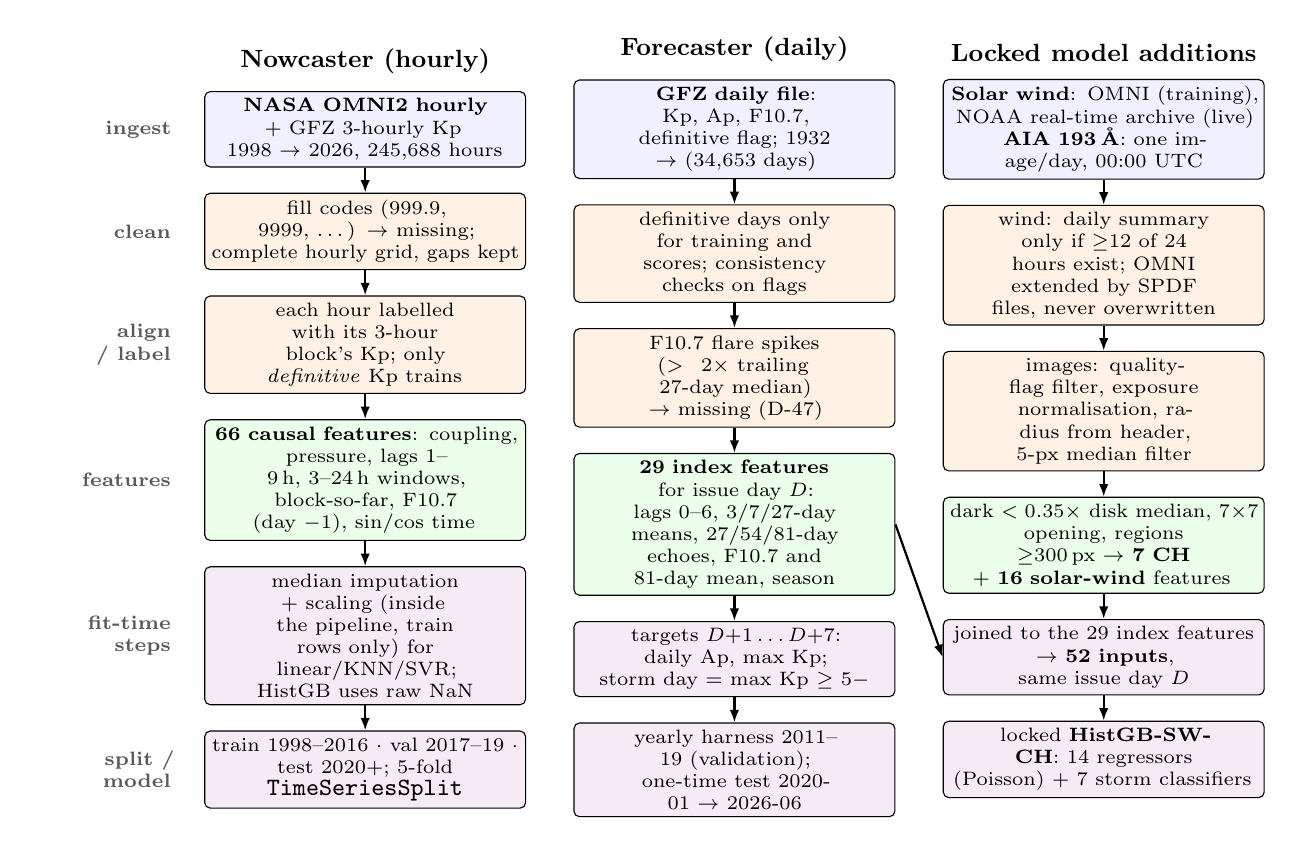
\begin{tikzpicture}[font=\scriptsize, node distance=3.2mm,
  stage/.style={font=\scriptsize\bfseries, text=gray!70!black, anchor=east, align=right, text width=1.7cm},
  box/.style={draw, rounded corners=2pt, align=center, text width=3.9cm, minimum height=7mm, inner sep=2.5pt},
  raw/.style={box, fill=blue!6}, cln/.style={box, fill=orange!10}, fea/.style={box, fill=green!8},
  mdl/.style={box, fill=violet!8}, ar/.style={-{Latex[length=1.6mm]}, thick}]
% column 1: nowcaster (hourly)
\node[raw] (o1) {\textbf{NASA OMNI2 hourly} + GFZ 3-hourly Kp\\1998 $\to$ 2026, 245{,}688 hours};
\node[cln, below=of o1] (o2) {fill codes (999.9, 9999, \ldots) $\to$ missing;\\complete hourly grid, gaps kept};
\node[cln, below=of o2] (o3) {each hour labelled with its 3-hour\\block's Kp; only \emph{definitive} Kp trains};
\node[fea, below=of o3] (o4) {\textbf{66 causal features}: coupling,\\pressure, lags 1--9\,h, 3--24\,h windows,\\block-so-far, F10.7 (day $-1$), sin/cos time};
\node[mdl, below=of o4] (o5) {median imputation + scaling (inside\\the pipeline, train rows only) for\\linear/KNN/SVR; HistGB uses raw NaN};
\node[mdl, below=of o5] (o6) {train 1998--2016 $\cdot$ val 2017--19 $\cdot$\\test 2020+; 5-fold \code{TimeSeriesSplit}};
% column 2: forecaster (daily)
\node[raw, right=6mm of o1] (d1) {\textbf{GFZ daily file}: Kp, Ap, F10.7,\\definitive flag; 1932 $\to$ (34{,}653 days)};
\node[cln, below=of d1] (d2) {definitive days only for training and\\scores; consistency checks on flags};
\node[cln, below=of d2] (d3) {F10.7 flare spikes ($>2\times$ trailing\\27-day median) $\to$ missing (D-47)};
\node[fea, below=of d3] (d4) {\textbf{29 index features} for issue day $D$:\\lags 0--6, 3/7/27-day means, 27/54/81-day\\echoes, F10.7 and 81-day mean, season};
\node[mdl, below=of d4] (d5) {targets $D{+}1\ldots D{+}7$: daily Ap, max Kp;\\storm day = max Kp $\ge$ 5$-$};
\node[mdl, below=of d5] (d6) {yearly harness 2011--19 (validation);\\one-time test 2020-01 $\to$ 2026-06};
% column 3: solar wind + images
\node[raw, right=6mm of d1] (s1) {\textbf{Solar wind}: OMNI (training),\\NOAA real-time archive (live)\\\textbf{AIA 193\,\AA}: one image/day, 00:00 UTC};
\node[cln, below=of s1] (s2) {wind: daily summary only if $\ge$12 of 24\\hours exist; OMNI extended by SPDF\\files, never overwritten};
\node[cln, below=of s2] (s3) {images: quality-flag filter, exposure\\normalisation, radius from header,\\5-px median filter};
\node[fea, below=of s3] (s4) {dark $<0.35\times$ disk median, $7{\times}7$\\opening, regions $\ge$300\,px $\to$ \textbf{7 CH}\\+ \textbf{16 solar-wind} features};
\node[mdl, below=of s4] (s5) {joined to the 29 index features\\$\to$ \textbf{52 inputs}, same issue day $D$};
\node[mdl, below=of s5] (s6) {locked \textbf{HistGB-SW-CH}: 14 regressors\\(Poisson) + 7 storm classifiers};
\foreach \c in {o,d,s}{\foreach \i/\j in {1/2,2/3,3/4,4/5,5/6}{\draw[ar] (\c\i) -- (\c\j);}}
\draw[ar] (d4.east) -- (s5.west);
% stage labels
\node[stage, left=3mm of o1] {ingest};
\node[stage, left=3mm of o2] {clean};
\node[stage, left=3mm of o3] {align / label};
\node[stage, left=3mm of o4] {features};
\node[stage, left=3mm of o5] {fit-time steps};
\node[stage, left=3mm of o6] {split / model};
\node[above=1mm of o1, font=\small\bfseries] {Nowcaster (hourly)};
\node[above=1mm of d1, font=\small\bfseries] {Forecaster (daily)};
\node[above=1mm of s1, font=\small\bfseries] {Locked model additions};
\end{tikzpicture}
\caption{Data pipeline from raw sources to model inputs. Blue: download; orange: cleaning and alignment (no fitted
parameters); green: features (causal, shared by training and live serving); violet: fitting and evaluation.}\label{fig:pipeline}
\end{figure}

\paragraph{Live and training paths are the same code.} One feature module per product computes features for training
and for the daily job, so they cannot diverge. Two parity checks confirm it:
\begin{itemize}
\item a nowcaster test shows identical features from the live and archive paths;
\item the near-real-time and archive images give identical coronal-hole features (Fig.~\ref{fig:live}).
\end{itemize}

%----------------------------------------------------------------------------------------------------------------
\section{System architecture}
Figure~\ref{fig:arch} shows the live system. Its design follows three rules:
\begin{itemize}
\item \textbf{One feature module per product, shared by training and live serving}, so features cannot be computed
differently in the two paths (a parity test checks this).
\item \textbf{Append-only logs.} Every forecast is written before its target day and never edited or backfilled.
\item \textbf{The issue job never fails because of an optional input.} Solar wind, images and NOAA products are each
wrapped so that a failure only warns, and the model falls back (\S\ref{sec:locked}).
\end{itemize}

\begin{figure}[htbp]\centering
\begin{tikzpicture}[font=\small, node distance=4mm and 7mm,
  src/.style={draw, rounded corners=2pt, fill=blue!6, minimum width=3.2cm, minimum height=7mm, align=center},
  job/.style={draw, rounded corners=2pt, fill=orange!10, minimum width=4.4cm, minimum height=7mm, align=center},
  out/.style={draw, rounded corners=2pt, fill=green!7, minimum width=3.6cm, minimum height=7mm, align=center},
  ar/.style={-{Latex[length=2mm]}, thick}]
\node[src] (gfz) {GFZ daily Kp/Ap/F10.7};
\node[src, below=of gfz] (sw) {NOAA real-time solar wind};
\node[src, below=of sw] (aia) {SDO/AIA 193\,\AA{} (JSOC NRT)};
\node[src, below=of aia] (noaa) {NOAA 3-day forecast, RSGA};

\node[job, right=12mm of gfz] (feat) {daily features (29)};
\node[job, right=12mm of sw] (swa) {solar-wind archive $\to$ 16 features};
\node[job, right=12mm of aia] (ch) {coronal-hole detection $\to$ 7 features};
\node[job, right=12mm of noaa] (bench) {benchmark store (never an input)};

\node[out, right=12mm of feat, yshift=-5mm] (live) {live HistGB + storm\\classifier + ARIMAX};
\node[out, below=of live] (lock) {locked HistGB-SW-CH\\(shadow, with fallbacks)};
\node[out, below=of lock] (score) {scoring vs GFZ and NOAA};

\draw[ar] (gfz) -- (feat); \draw[ar] (sw) -- (swa); \draw[ar] (aia) -- (ch); \draw[ar] (noaa) -- (bench);
\draw[ar] (feat) -- (live); \draw[ar] (feat.east) -- (lock.west);
\draw[ar] (swa.east) -- (lock.west); \draw[ar] (ch.east) -- (lock.west);
\draw[ar] (live) -- (lock); \draw[ar] (lock) -- (score); \draw[ar] (bench.east) -- (score.west);
\begin{scope}[on background layer]
\node[draw=gray, dashed, rounded corners, fit=(feat)(bench)(live)(score), inner sep=3mm,
      label={[gray]above:daily GitHub Actions job (\code{src/issue.py}), several overnight slots}] {};
\end{scope}
\node[below=6mm of score, align=center, text width=8.5cm, font=\footnotesize] (logs)
 {append-only logs in \code{forecasts/} $\to$ Streamlit app, Hugging Face Space and model repository};
\draw[ar] (score) -- (logs);
\end{tikzpicture}
\caption{Live forecaster architecture. The nowcaster runs separately: NOAA solar wind $\to$ 66 hourly features
$\to$ HistGB with conformal quantile interval, refreshed every hour and logged.}\label{fig:arch}
\end{figure}

\paragraph{Shadow mode.} A candidate runs every day next to the live model. Its forecasts are logged and scored,
but not shown. This is the only way to test what a validation run cannot:
\begin{itemize}
\item real-time inputs (NOAA's feed and JSOC's near-real-time images) instead of corrected archives;
\item a solar-wind archive that only reaches 27 days of history after 27 days of operation;
\item fallbacks triggered by real outages.
\end{itemize}
D-69 showed why this matters: with the solar-wind feed down, the solar-wind model scores \emph{below} the live model
(Ap skill 0.075 vs 0.089), so a silent outage would make forecasts worse.

%----------------------------------------------------------------------------------------------------------------
\section{Features}
\subsection{Nowcaster: 66 hourly features}
The nowcaster computes 66 causal features from 8 raw inputs ($|B|$, $B_x$, $B_y$, $B_z$, speed, density,
temperature, F10.7):
\begin{itemize}
\item coupling functions: $-VB_z$, $VB_s$, Newell \cite{newell2007};
\item pressure, plasma $\beta$ and Alfv\'en Mach number;
\item lags of 1--9\,h, and 3--24\,h windows (means, spread and extremes);
\item statistics since the current 3-hour block began;
\item previous-day F10.7 and its 81-day mean;
\item hour of day and day of year as sin/cos, which carries the Russell--McPherron effect \cite{russell1973}.
\end{itemize}
No geomagnetic index is an input.

\subsection{Forecaster: 29 + 16 + 7 = 52 daily features}
\begin{table}[htbp]\centering\small
\caption{Forecaster inputs for issue day $D$ and lead day $h$. Each group is a strict superset of the one above it.}\label{tab:feat}
\begin{tabularx}{\textwidth}{@{}p{3.1cm}cY@{}}\toprule
Group & \# & Features\\\midrule
Indices (live HistGB) & 29 & Ap and max Kp of $D$ and the 6 days before (14); 3/7/27-day Ap means, 7-day Ap s.d., 27-day max-Kp mean, 7-day max-Kp max; F10.7 (flare spikes filtered) and its 81-day mean; 27-day echo of Ap (and $\pm$1-day mean) and max Kp, Ap 54 and 81 days before the target; day of year (sin, cos)\\
Solar wind (D-68) & 16 & daily speed (mean, max), $B_z$ (mean, min), $VB_s$, density, $|B|$, peak pressure and $B_y$ for $D$; speed and $VB_s$ for $D-1$; speed change; 27-day echo of speed ($\pm$1-day mean), maximum speed and $B_y$ for the target day\\
Coronal holes (D-70) & 7 & low-latitude Earth-facing hole area on $D$, $D-1$, $D-2$ and its change since $D-1$; incoming (east-limb) area; whole-disk area; mean darkness\\\bottomrule
\end{tabularx}
\end{table}

\paragraph{Coronal-hole detection.} The detection uses no learned parameters.
\begin{enumerate}
\item Each 00:00 UTC 193\,\AA{} image is normalised by exposure time.
\item On-disk pixels ($r<0.95\,R_\odot$, with $R_\odot=$ \code{RSUN\_OBS}/\code{CDELT1}) count as dark if they fall
below $0.35\times$ the disk median after a 5-pixel median filter.
\item The dark mask is cleaned with a $7\times7$ opening, and regions under 300 pixels (mostly filaments) are
removed.
\end{enumerate}
The ``Earth-facing, low-latitude'' strip is $|x|<0.3\,R_\odot$, $|y|<0.5\,R_\odot$ (Fig.~\ref{fig:ch}). Coronal
holes emit fast wind that reaches Earth 2--4 days after crossing the central meridian
\cite{krieger1973,vrsnak2007a,rotter2012}. Our data show exactly this: the correlation of strip area with
solar-wind speed peaks at 3--4 days and with Ap at 3 days (Fig.~\ref{fig:chlag}), consistent with the 4-day
geomagnetic peak found by \cite{vrsnak2007b}.

\begin{figure}[htbp]\centering
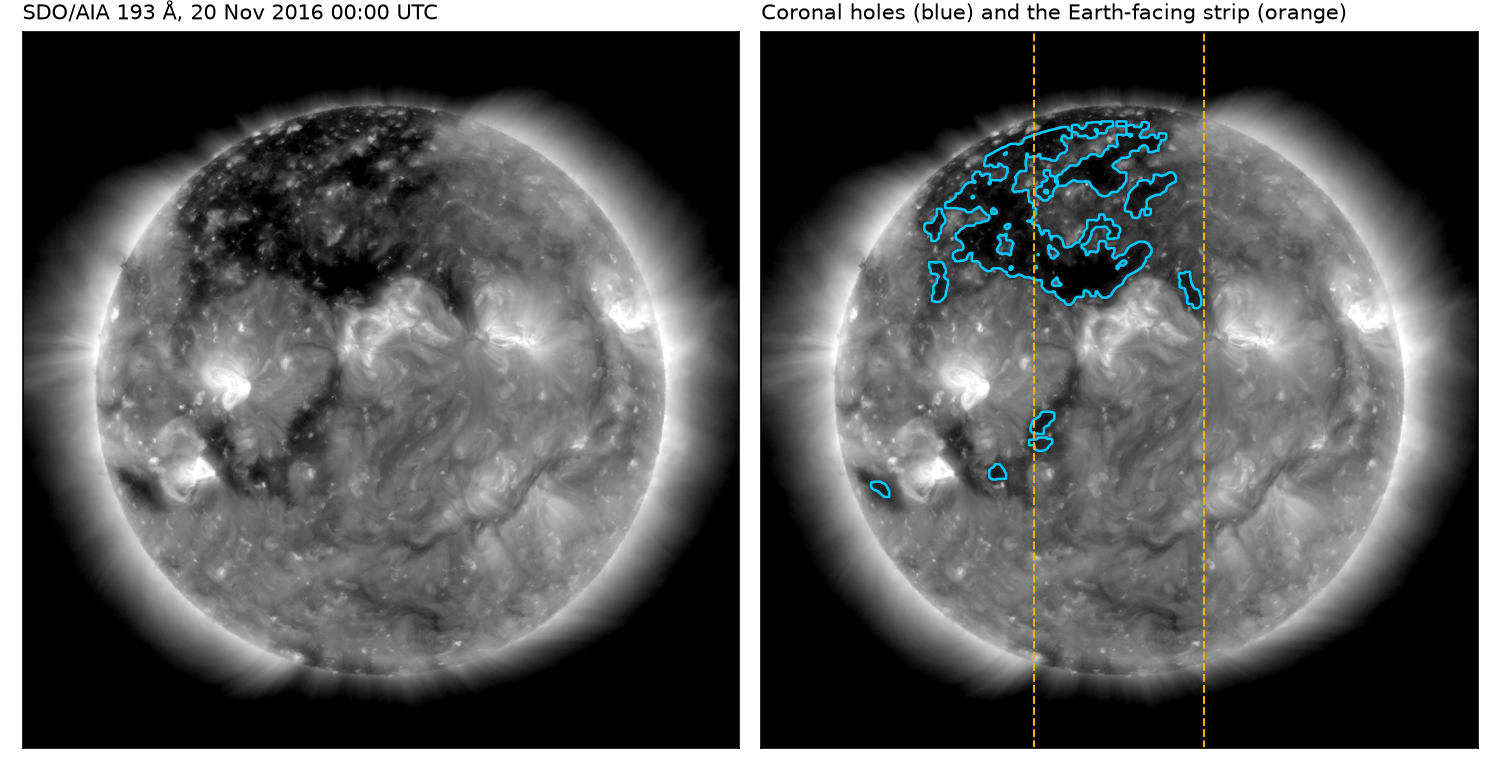
\includegraphics[width=0.9\textwidth]{fc_08_coronal_hole_example.png}
\caption{AIA 193\,\AA{} image of 20 Nov 2016 (left) and the detected coronal holes with the Earth-facing strip
(right).}\label{fig:ch}
\end{figure}
\begin{figure}[htbp]\centering
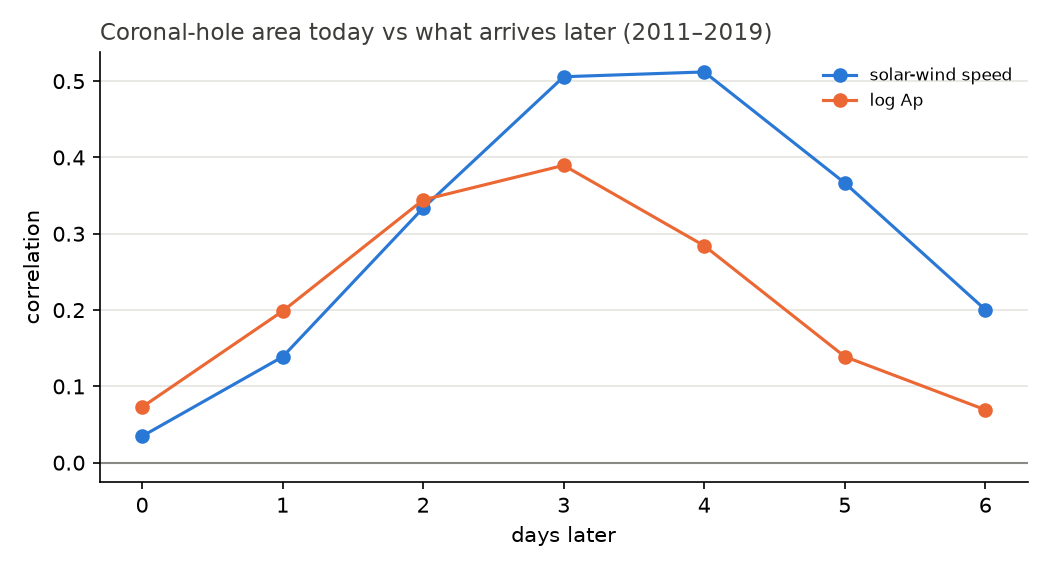
\includegraphics[width=0.62\textwidth]{fc_10_coronal_holes_vs_wind.png}
\caption{Correlation of the Earth-facing coronal-hole area on day $D$ with daily solar-wind speed and log Ap on day
$D+k$, 2011--2019. Both peak 3--4 days later, the travel time of fast wind.}\label{fig:chlag}
\end{figure}

%----------------------------------------------------------------------------------------------------------------
\section{Evaluation design}\label{sec:eval}
\begin{itemize}
\item \textbf{Skill} $=1-\mathrm{SSE}_{\text{model}}/\mathrm{SSE}_{\text{27-day mean}}$ per lead day, averaged over
days 1--7. The 27-day trailing mean is the hardest of our four reference forecasts.
\item \textbf{Storm warnings} use the Heidke skill score (HSS), probability of detection (POD) and false-alarm
ratio (FAR) \cite{wilks2011}. Warning thresholds are tuned for the rare event on training or harness years only.
\item \textbf{Yearly harness (D-68).} For each year 2011--2019, train on every day before it and forecast that year.
This gives 9 years, 362 storm days and a full solar cycle. A change is kept only if, by a rule written before the
run:
  \begin{enumerate}
  \item pooled skill improves;
  \item it wins in at least 6 of 9 years (by chance about 25\% of the time);
  \item storm Heidke for days 1--3 does not fall by more than 0.01.
  \end{enumerate}
  Image changes are judged on 2013--2019, 5 of 7 years.
\item \textbf{Test.} Scored once after the lock. Significance comes from the Diebold--Mariano test on squared Ap
errors \cite{diebold1995} with Newey--West variance, lag $h-1$ \cite{newey1987}, and a 30-day block bootstrap
\cite{kunsch1989} of the skill difference.
\item \textbf{No future data.} Tests delete everything after the issue day and check that the forecast is unchanged.
Image features for day $D$ come only from the 00:00 UTC image of $D$ or earlier.
\end{itemize}

%----------------------------------------------------------------------------------------------------------------
\section{Models tried}
\begin{table}[htbp]\centering\small
\caption{Every model family tried, on the period where it was compared. ``Kept'' means it passed its pre-set rule.}\label{tab:models}
\begin{tabularx}{\textwidth}{@{}p{3.6cm}p{2.3cm}Yc@{}}\toprule
Model & Product & Result & Kept\\\midrule
Persistence & nowcast & test RMSE 0.862 & reference\\
Linear regression & nowcast & 0.665 & --\\
KNN & nowcast & 0.657 (memorises: train RMSE $\approx$0) & --\\
SVR (RBF) & nowcast & 0.605 & --\\
Random forest & nowcast & 0.606 & --\\
\textbf{HistGB} \cite{ke2017,pedregosa2011} & nowcast & \textbf{0.573}, $R^2$ 0.808 & \checkmark\\\midrule
ARIMA / SARIMA \cite{box2015} & forecast & test skill 0.062 / 0.025 & --\\
ARIMAX & forecast & 0.069 & \checkmark\ (comparison)\\
Chronos-Bolt, zero-shot \cite{ansari2024} & forecast & $-0.015$ & --\\
Holt--Winters \cite{winters1960} & forecast & harness $-0.108$ & --\\
LSTM \cite{hochreiter1997} & forecast & harness 0.029 & --\\
GRU \cite{cho2014} & forecast & harness 0.051 & --\\
\textbf{HistGB direct} (14 models) & forecast & test 0.100, harness 0.089 & \checkmark\ (live)\\
HistGB + solar wind + echo, Poisson & forecast & harness 0.112, 9/9 years & candidate\\
\textbf{HistGB-SW-CH} & forecast & test \textbf{0.122}; harness 0.160 (2013--19, 7/7) & \checkmark\ (locked)\\\bottomrule
\end{tabularx}
\end{table}

Gradient boosting with hand-built features beats both recurrent networks on the same days
(Fig.~\ref{fig:valmodels}). With about 23{,}000 daily samples and a few dozen inputs, trees extract more than
sequence models, which also need far more tuning. Holt--Winters follows day-to-day noise and is worse than the 27-day
mean.

\begin{figure}[htbp]\centering
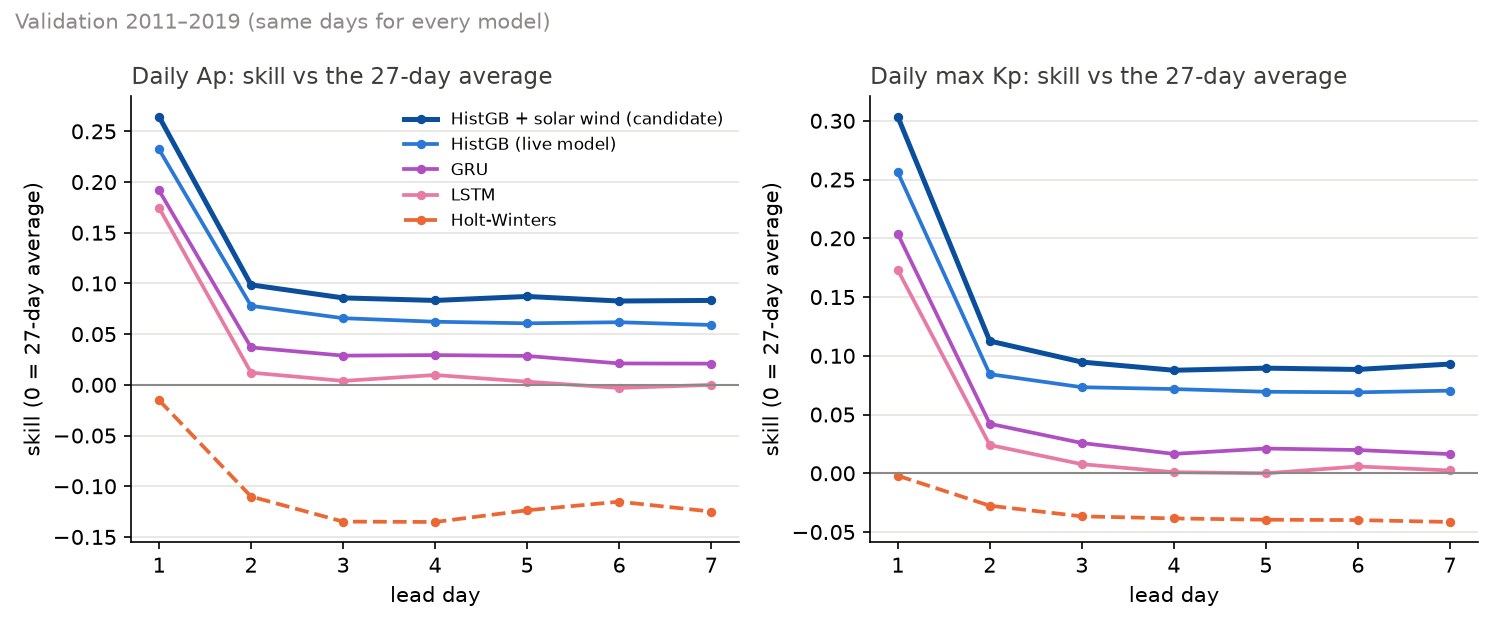
\includegraphics[width=\textwidth]{fc_05_validation_models.png}
\caption{Model families on the yearly harness (2011--2019), Ap skill by lead day (D-75).}\label{fig:valmodels}
\end{figure}

%----------------------------------------------------------------------------------------------------------------
\section{The locked model and its parameters}\label{sec:locked}
\textbf{HistGB-SW-CH} (D-76) consists of:
\begin{itemize}
\item 14 regressors, one per lead day (1--7) and target (Ap, max Kp), so errors never feed forward;
\item 7 storm classifiers on the same 52 inputs.
\end{itemize}
Its settings were not retuned for the new inputs (Table~\ref{tab:params}), so no settings were chosen on the
harness.

\begin{table}[htbp]\centering\small
\caption{Locked model settings (scikit-learn \code{HistGradientBoosting*}, \code{early\_stopping=False}, seed 42).}\label{tab:params}
\begin{tabular}{@{}lccc@{}}\toprule
 & Ap regressor & max-Kp regressor & storm classifier\\\midrule
loss & Poisson & Poisson & log loss\\
learning rate & 0.03 & 0.02 & 0.05\\
iterations & 200 & 400 & 300\\
max leaf nodes & 7 & 7 & 15\\
min samples per leaf & 200 & 400 & 100\\
L2 regularisation & 3.0 & 3.0 & 1.0\\
how chosen & \multicolumn{2}{c}{tuned on 1947--2016 (D-31), then frozen} & fixed in advance (D-48)\\
warning thresholds & \multicolumn{3}{c}{per lead day, max Heidke on harness probabilities 2011--2019}\\\bottomrule
\end{tabular}
\end{table}

\paragraph{Fallbacks (logged on every row).} If no usable image exists for $D$ or $D-1$, the solar-wind model is
served. If there is no solar wind for $D$, the live HistGB is served.

\paragraph{Why each input group passed.}
\begin{itemize}
\item \textbf{Solar wind and echo (D-68).} Ap skill 0.089 $\to$ 0.112, max-Kp skill 0.099 $\to$ 0.124, 9 of 9 years.
The gain is spread over every lead day: the stream passing on day $D$ indicates how long the disturbance lasts, and
the 27-day echo marks recurring fast streams.
\item \textbf{Coronal holes (D-70), 2013--2019.} Ap skill 0.131 $\to$ 0.160, days 2--4 0.110 $\to$ 0.155, 7 of 7
years, storm Heidke 0.310 $\to$ 0.364. The gain is largest on days 2--5, the travel time of fast wind.
\item \textbf{Leakage controls (fixed before running).} Using the previous day's image keeps most of the gain (0.154).
Images placed on random days lose it (0.137, 4 of 7 years). The gain therefore comes from real images on their real
dates.
\item \textbf{Live inputs.} JSOC near-real-time images and archive images give identical features (correlation 1.000
over 30 days, Fig.~\ref{fig:live}).
\end{itemize}

\begin{figure}[htbp]\centering
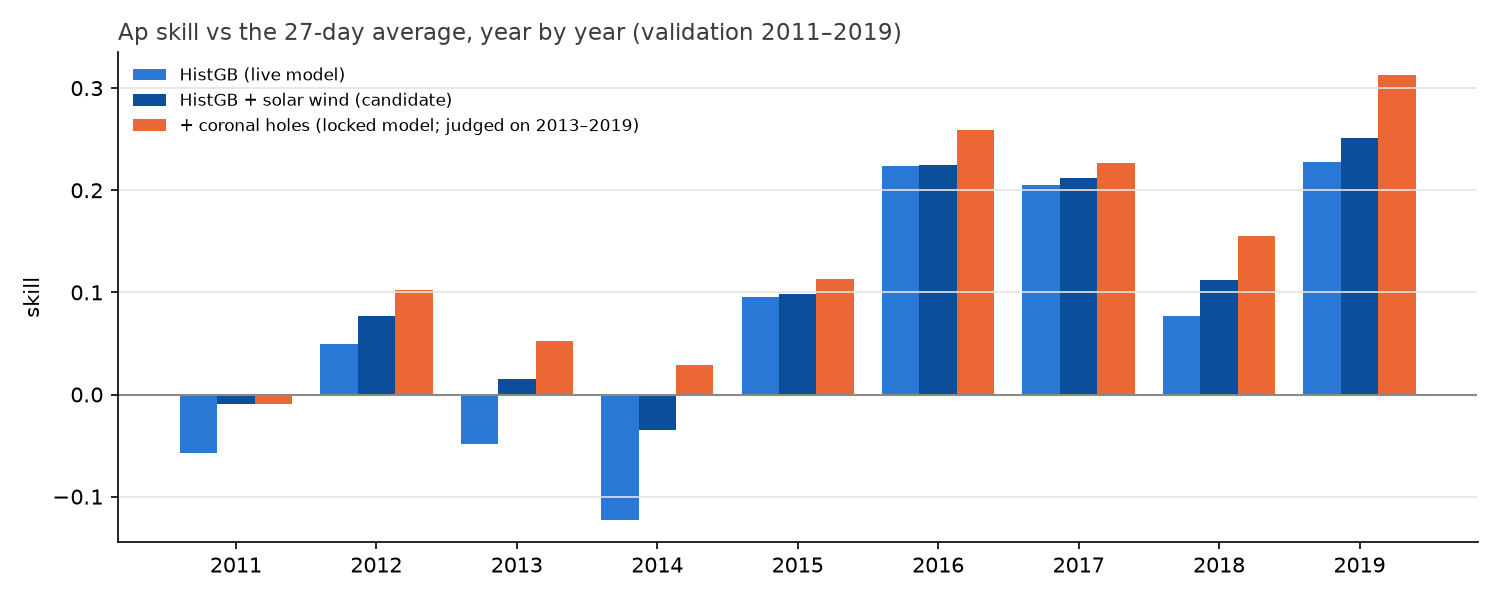
\includegraphics[width=\textwidth]{fc_06_validation_by_year.png}
\caption{Ap skill per harness year: live HistGB, solar-wind candidate and locked model.}\label{fig:byyear}
\end{figure}
\begin{figure}[htbp]\centering
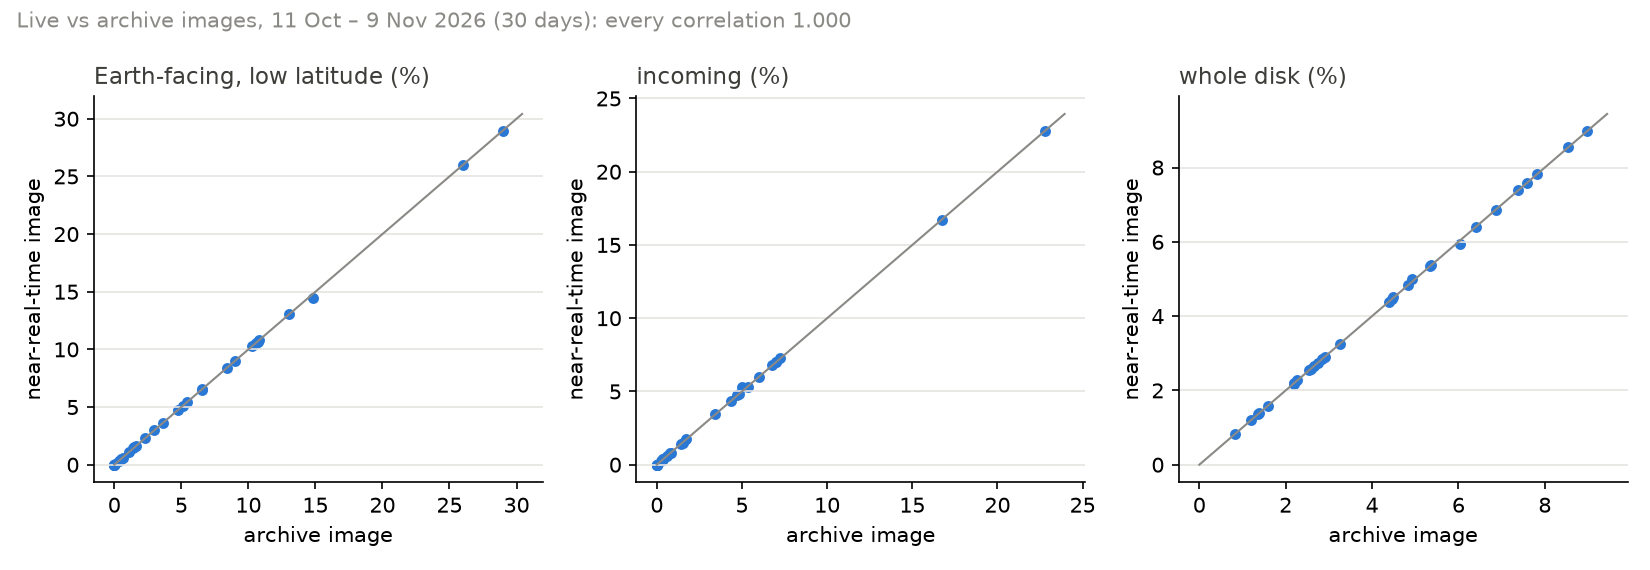
\includegraphics[width=\textwidth]{fc_09_live_vs_archive_images.png}
\caption{Coronal-hole features from near-real-time vs archive images on the same 30 days.}\label{fig:live}
\end{figure}

%----------------------------------------------------------------------------------------------------------------
\section{Decisions and their reasons}
DECISIONS.md records 77 decisions, each with its rule and result; failures are kept on record. Table~\ref{tab:dec}
lists those that shaped the system.

{\small
\begin{longtable}{@{}p{1.3cm}p{5.6cm}p{9.4cm}@{}}
\caption{Key decisions (D-numbers refer to DECISIONS.md).}\label{tab:dec}\\\toprule
ID & Decision & Reason\\\midrule\endfirsthead
\toprule ID & Decision & Reason\\\midrule\endhead
v1 & No geomagnetic index as nowcaster input & the nowcast must not wait for magnetometers; an ablation showed past Kp would add only 0.010 RMSE\\
v1 & Hourly rows labelled with their 3-hour block's Kp & the live app runs mid-block; training on whole blocks would use unavailable data\\
v1 & Conformal correction of quantile models \cite{romano2019} & raw quantiles covered 75.7\%; corrected 80.8\%\\
D-02 & Past Kp/Ap allowed for the forecaster & beyond a day, past activity and the 27-day rotation are the information left\\
D-03 & Targets: daily Ap and max Kp & what NOAA forecasts, so the comparison is direct\\
D-06 & NOAA is a benchmark, never an input & otherwise our skill would be borrowed\\
D-19 & Train from 1947-06-01 & the first day every input exists; D-66 confirmed shorter history is worse\\
D-22/48 & Separate storm classifier, rare-event thresholds, no resampling & mean forecasts rarely cross the storm line; resampling distorts probabilities\\
D-27/63 & Live models frozen on a fixed window & forecasts change only when inputs change\\
D-31 & Direct models, one per lead day & a recursive model feeds on its own errors\\
D-51/52 & Models committed before the test; test scored once & git history proves the test did not influence the choice\\
D-62 & One re-score after a pre-test bug audit & the fix came before any new test number; reported whatever it showed\\
D-67 & CME catalogue rejected & starts 2014; added almost nothing, hurt storm Heidke\\
D-68 & Yearly harness, rules fixed in advance & one 3-year solar-minimum block was too short to judge small changes\\
D-69 & Shadow mode and fallback & with the feed down the solar-wind model is worse than the live model\\
D-70 & Coronal holes from one image per day, no deep network & coronal holes drive days 2--5; ~3{,}500 images is too few to train a CNN\\
D-72--74 & Intraday reissue, issue-day state, flare signs rejected & each caught more storms only by warning more often\\
D-76 & Lock and test protocol fixed before test data & further experiments on the same years add selection risk\\
D-77 & One-time test of the locked model & adoption rules (a) and (b) pass; level with NOAA; recorded as it came out\\\bottomrule
\end{longtable}}

%----------------------------------------------------------------------------------------------------------------
\section{Results}
\subsection{Nowcaster (test 2020--Jan 2026)}
HistGB reaches RMSE 0.573 Kp ($R^2$ 0.808), 34\% below persistence overall and 38\% on storm hours. The 80\%
interval covers 80.8\% of test hours, and the live RMSE against GFZ quick-look Kp is about 0.59.
Fig.~\ref{fig:may} shows the May 2024 G5 storm: the predicted peak is 8.6 against an observed 9.

\begin{figure}[htbp]\centering
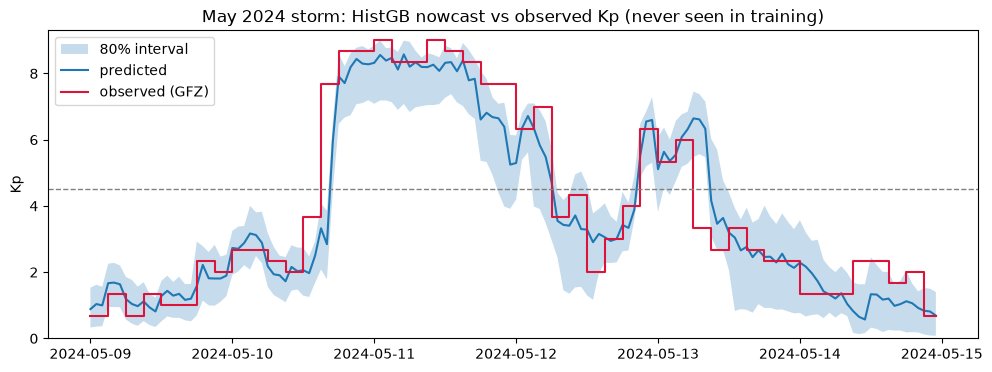
\includegraphics[width=0.92\textwidth]{14_may2024_nowcast.png}
\caption{Nowcast of the May 2024 storm (never seen in training) with its 80\% interval.}\label{fig:may}
\end{figure}

\subsection{Forecaster: v2.0 live model on the test period (D-62)}
\begin{table}[htbp]\centering\small
\caption{Daily Ap RMSE on the test period (2,379 days); skill vs the 27-day mean, days 1--7.}\label{tab:v2test}
\begin{tabular}{@{}lcccc@{}}\toprule
Model & day 1 & day 3 & day 7 & skill\\\midrule
HistGB (live v2.0) & \textbf{10.78} & 11.91 & \textbf{12.01} & \textbf{+0.100}\\
NOAA official & 10.89 & \textbf{11.90} & -- & +0.134 (days 1--3)\\
ARIMAX & 10.96 & 12.15 & 12.17 & +0.069\\
Chronos-Bolt & 11.83 & 12.66 & 12.65 & $-0.015$\\
27-day mean & 12.27 & 12.45 & 12.48 & 0\\\bottomrule
\end{tabular}
\end{table}

\subsection{Locked model on the test period (D-77)}
The locked model was fitted on 1947-06 to 2019 and forecast every day of the test period once (D-76 protocol).
All test scores in this report come from models fitted only on data up to 2019. After scoring, the deployed models
(nowcaster, live forecaster and locked model) were refitted on all definitive data up to June 2026, test years
included. Their only out-of-sample evidence from then on is the live and shadow logs.
Coronal-hole features exist for 2{,}360 of the 2{,}373 days; the 13 days without a usable image keep blank image
inputs. Table~\ref{tab:locked} and Fig.~\ref{fig:locked} give the result.

\begin{table}[htbp]\centering\small
\caption{One-time test, 2020-01-01 to 2026-06-30 (2,373 days, 325 storm days). Daily Ap RMSE; DM = Diebold--Mariano
test of the locked model against the live HistGB on the same days (negative = locked better). NOAA is scored on the
days it issued (2,358--2,359).}\label{tab:locked}
\setlength{\tabcolsep}{5pt}
\begin{tabular}{@{}lccccccc@{}}\toprule
Lead day & 1 & 2 & 3 & 4 & 5 & 6 & 7\\\midrule
\textbf{Locked HistGB-SW-CH} & \textbf{10.67} & 11.80 & \textbf{11.73} & \textbf{11.69} & \textbf{11.72} & \textbf{11.88} & \textbf{11.95}\\
Live HistGB & 10.78 & 11.98 & 11.91 & 11.91 & 11.93 & 11.96 & 12.01\\
NOAA official & 10.89 & \textbf{11.73} & 11.90 & -- & -- & -- & --\\
27-day mean & 12.27 & 12.42 & 12.45 & 12.45 & 12.45 & 12.46 & 12.48\\\midrule
DM statistic & $-1.69$ & $-2.77$ & $-2.25$ & $-2.98$ & $-3.78$ & $-1.44$ & $-1.40$\\
DM $p$ & 0.091 & 0.006 & 0.025 & 0.003 & $<$0.001 & 0.149 & 0.161\\\midrule
Max-Kp RMSE, locked & 1.115 & 1.221 & 1.225 & 1.226 & 1.232 & 1.242 & 1.246\\
Max-Kp RMSE, live & 1.138 & 1.250 & 1.256 & 1.257 & 1.259 & 1.257 & 1.260\\\midrule
Heidke, locked & \textbf{0.403} & \textbf{0.263} & \textbf{0.249} & \textbf{0.221} & 0.209 & \textbf{0.206} & \textbf{0.222}\\
Heidke, live & 0.341 & 0.195 & 0.204 & 0.205 & \textbf{0.215} & 0.202 & 0.188\\
POD / FAR, locked & 53/54\% & 40/65\% & 31/62\% & 29/65\% & 36/70\% & 54/74\% & 34/68\%\\
POD / FAR, live & 47/59\% & 38/72\% & 30/68\% & 46/73\% & 43/71\% & 46/73\% & 24/66\%\\\bottomrule
\end{tabular}
\end{table}

\begin{figure}[htbp]\centering
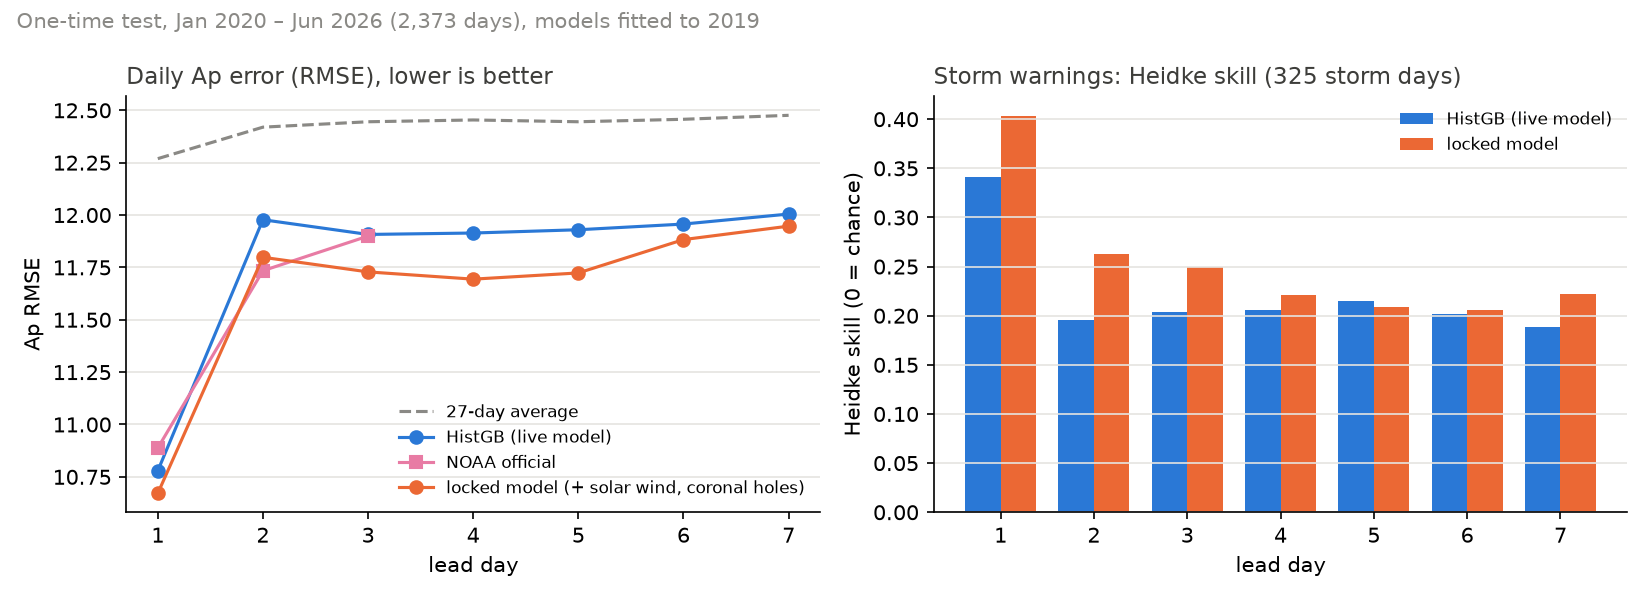
\includegraphics[width=\textwidth]{fc_11_locked_test_vs_noaa.png}
\caption{One-time test: daily Ap error by lead day (left) and storm-warning Heidke skill (right).}\label{fig:locked}
\end{figure}

\begin{itemize}
\item \textbf{Skill vs the 27-day mean (days 1--7):} 0.122 against 0.100 for the live HistGB (+22\%). The 30-day
block bootstrap puts the gain between $+0.007$ and $+0.050$ (95\%), so it is not chance.
\item \textbf{Where the gain is:} days 2--5 are significantly better ($p\le0.025$), the travel time of fast wind from
a coronal hole, as on validation. Days 1, 6 and 7 are better but not significantly.
\item \textbf{Storm warnings:} mean Heidke on days 1--3 rises from 0.247 to 0.305, with fewer false alarms and
slightly more storms caught. The rejected storm experiments (D-72 to D-74) caught more only by warning more.
\item \textbf{Adoption rule (D-76):} (a) better pooled skill and day-1 RMSE: pass; (b) storm Heidke days 1--3 not
lower: pass; (c) three weeks of shadow running with working fallbacks: in progress.
\item \textbf{Smaller than on validation:} the test years include the rise to the 2024 solar maximum, when CME
storms, which none of our inputs see in advance, are more frequent; this is the likely reason the gain is smaller
than on 2013--2019.
\end{itemize}

%----------------------------------------------------------------------------------------------------------------
\section{Comparison with NOAA}\label{sec:noaa}
NOAA SWPC's forecasts are issued by human forecasters who watch the Sun directly, including CME launches and
coronagraph data. Two comparisons exist:
\begin{itemize}
\item \textbf{Storm warnings, 2017--2019} (91 storm days, Fig.~\ref{fig:noaastorm}). NOAA's Heidke is 0.41 / 0.38 /
0.32 on days 1/2/3, against 0.40 / 0.34 / 0.34 for the solar-wind candidate. We catch more storm days but raise
more false alarms.
\item \textbf{Ap values on the test period} (2,358--2,359 days, Table~\ref{tab:locked}). The locked model is ahead on
day 1 (10.66 vs 10.89) and day 3 (11.67 vs 11.90) and behind on day 2 (11.82 vs 11.73). Diebold--Mariano $p$ =
0.69 / 0.91 / 0.55: \textbf{no significant difference}. The live HistGB was already level with NOAA (D-62); the
locked model stays level with NOAA while being significantly better than the live model.
\end{itemize}

\begin{figure}[htbp]\centering
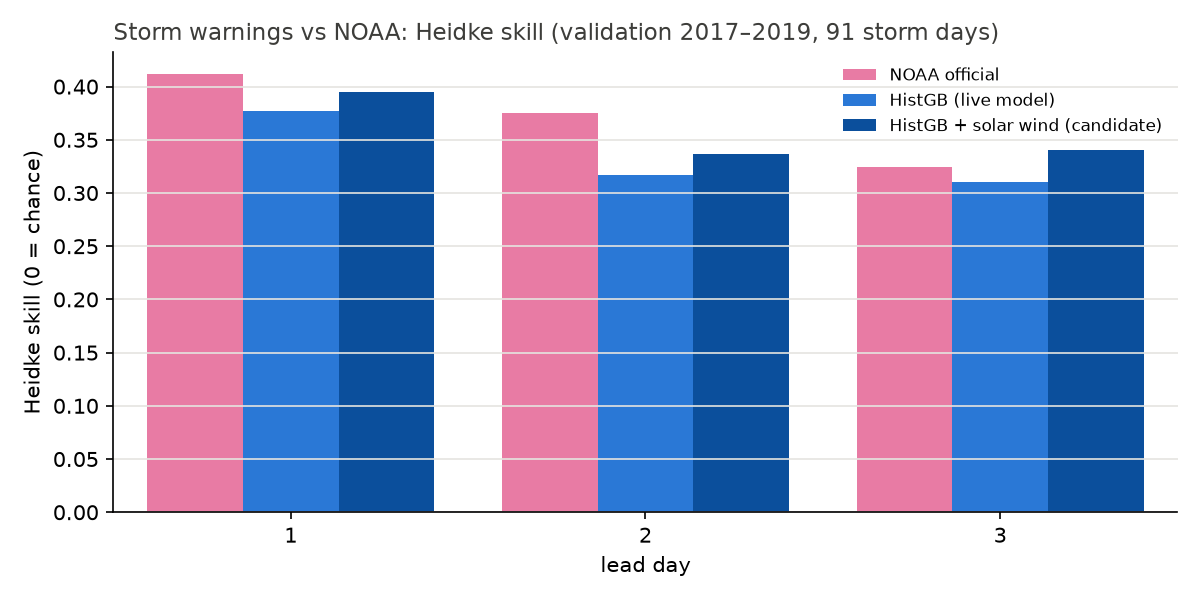
\includegraphics[width=0.8\textwidth]{fc_07_storms_vs_noaa.png}
\caption{Storm-warning Heidke skill vs NOAA, 2017--2019 (D-71).}\label{fig:noaastorm}
\end{figure}

\paragraph{Paper decision (guide fixed before the test, ROADMAP \S8).}
\begin{itemize}
\item Significantly better than NOAA on days 1--3 $\Rightarrow$ journal paper (e.g.\ \emph{Space Weather}).
\item Level with NOAA and significantly better than the live model $\Rightarrow$ solid paper. The contribution is a
transparent, reproducible, image-plus-index model that matches the operational forecast.
\item Behind $\Rightarrow$ workshop paper or report only.
\end{itemize}
\textbf{Outcome: the middle case, a solid paper.} The model is level with NOAA's human-in-the-loop forecast on days
1--3 using only public data and one image per day, significantly better than an index-only model on days 2--5, and
the gain is traced to coronal holes by a lag and a placebo control. Related ML work on Kp \cite{zhelavskaya2019,camporeale2019} mostly targets hours ahead from solar
wind. Coronal-hole forecasting \cite{rotter2015,vrsnak2007a} mostly predicts wind speed. A multi-day Ap forecaster
that combines both, scored against NOAA under a pre-registered protocol, is the gap this work could fill.

%----------------------------------------------------------------------------------------------------------------
\section{Deployment}
\begin{itemize}
\item \textbf{Streamlit app} (\url{https://tormenta.streamlit.app/}) has six pages:
  \begin{itemize}
  \item Overview, Forecast and Nowcast;
  \item Explore, which replays any past issue day;
  \item Scorecard, which shows every model with its figures;
  \item Method.
  \end{itemize}
  It is shown in Pakistan time, with light and dark themes.
\item \textbf{Daily GitHub Actions job}, run in several overnight slots, does the following:
  \begin{itemize}
  \item issues the forecast;
  \item archives the solar wind and the near-real-time AIA image features;
  \item logs the shadow models;
  \item scores every forecast whose day has arrived;
  \item stores NOAA's products.
  \end{itemize}
  A failure in any optional step only warns.
\item \textbf{Weekly retrain check} retrains only after two degraded health checks in a row, and promotes a new model
only if it beats the current one on recent unseen data.
\item \textbf{Hugging Face} hosts the model repository with its model card, and an in-browser Space.
\end{itemize}

%----------------------------------------------------------------------------------------------------------------
\section{Limitations}
\begin{itemize}
\item \textbf{CME storms} leave no trace in past indices or in coronal holes until they arrive. Their first day is
usually missed: on 10 May 2024 the onset was missed, and the next three storm days were warned.
\item \textbf{Storm size is under-predicted}, because Kp\,9 days are very rare in training. During storms the warning
is the number to trust.
\item \textbf{Validation years.} 2017--2019 is solar minimum, and the NOAA storm comparison rests on 91 storm days.
\item \textbf{Image availability.} Live images come only from JSOC's near-real-time folder. A gap of two days
switches the forecast to the solar-wind model.
\item This is a course project, not an operational warning service.
\end{itemize}

%----------------------------------------------------------------------------------------------------------------
{\small
\begin{thebibliography}{30}\setlength{\itemsep}{0pt}
\bibitem{matzka2021} J.~Matzka, C.~Stolle, Y.~Yamazaki, O.~Bronkalla and A.~Morschhauser, ``The geomagnetic Kp index and derived indices of geomagnetic activity,'' \emph{Space Weather}, 19, e2020SW002641, 2021.
\bibitem{gfzkp} J.~Matzka, O.~Bronkalla, K.~Tornow, K.~Elger and C.~Stolle, \emph{Geomagnetic Kp index}, V.~1.0, GFZ Data Services, 2021, doi:10.5880/Kp.0001.
\bibitem{king2005} J.~H. King and N.~E. Papitashvili, ``Solar wind spatial scales in and comparisons of hourly Wind and ACE plasma and magnetic field data,'' \emph{J. Geophys. Res.}, 110, A02104, 2005.
\bibitem{swpc} NOAA Space Weather Prediction Center, real-time solar wind, 3-day forecast and RSGA products, \url{https://www.swpc.noaa.gov}.
\bibitem{lemen2012} J.~R. Lemen et al., ``The Atmospheric Imaging Assembly (AIA) on the Solar Dynamics Observatory (SDO),'' \emph{Solar Physics}, 275, 17--40, 2012.
\bibitem{pesnell2012} W.~D. Pesnell, B.~J. Thompson and P.~C. Chamberlin, ``The Solar Dynamics Observatory (SDO),'' \emph{Solar Physics}, 275, 3--15, 2012.
\bibitem{newell2007} P.~T. Newell, T.~Sotirelis, K.~Liou, C.-I. Meng and F.~J. Rich, ``A nearly universal solar wind-magnetosphere coupling function inferred from 10 magnetospheric state variables,'' \emph{J. Geophys. Res.}, 112, A01206, 2007.
\bibitem{russell1973} C.~T. Russell and R.~L. McPherron, ``Semiannual variation of geomagnetic activity,'' \emph{J. Geophys. Res.}, 78(1), 92--108, 1973.
\bibitem{krieger1973} A.~S. Krieger, A.~F. Timothy and E.~C. Roelof, ``A coronal hole and its identification as the source of a high velocity solar wind stream,'' \emph{Solar Physics}, 29, 505--525, 1973.
\bibitem{vrsnak2007a} B.~Vr\v{s}nak, M.~Temmer and A.~M. Veronig, ``Coronal holes and solar wind high-speed streams: I.~Forecasting the solar wind parameters,'' \emph{Solar Physics}, 240, 315--330, 2007, doi:10.1007/s11207-007-0285-8.
\bibitem{vrsnak2007b} B.~Vr\v{s}nak, M.~Temmer and A.~M. Veronig, ``Coronal holes and solar wind high-speed streams: II.~Forecasting the geomagnetic effects,'' \emph{Solar Physics}, 240, 331--346, 2007.
\bibitem{rotter2012} T.~Rotter, A.~M. Veronig, M.~Temmer and B.~Vr\v{s}nak, ``Relation between coronal hole areas on the Sun and the solar wind parameters at 1~AU,'' \emph{Solar Physics}, 281, 793--813, 2012.
\bibitem{rotter2015} T.~Rotter, A.~M. Veronig, M.~Temmer and B.~Vr\v{s}nak, ``Real-time solar wind prediction based on SDO/AIA coronal hole data,'' \emph{Solar Physics}, 290, 1355--1370, 2015.
\bibitem{zhelavskaya2019} I.~S. Zhelavskaya, R.~Vasile, Y.~Y. Shprits, C.~Stolle and J.~Matzka, ``Systematic analysis of machine learning and feature selection techniques for prediction of the Kp index,'' \emph{Space Weather}, 17, 1461--1486, 2019.
\bibitem{camporeale2019} E.~Camporeale, ``The challenge of machine learning in space weather: Nowcasting and forecasting,'' \emph{Space Weather}, 17, 1166--1207, 2019.
\bibitem{ke2017} G.~Ke et al., ``LightGBM: A highly efficient gradient boosting decision tree,'' \emph{NeurIPS}, 2017.
\bibitem{pedregosa2011} F.~Pedregosa et al., ``Scikit-learn: Machine learning in Python,'' \emph{JMLR}, 12, 2825--2830, 2011.
\bibitem{romano2019} Y.~Romano, E.~Patterson and E.~Cand\`es, ``Conformalized quantile regression,'' \emph{NeurIPS}, 2019.
\bibitem{box2015} G.~E.~P. Box, G.~M. Jenkins, G.~C. Reinsel and G.~M. Ljung, \emph{Time Series Analysis: Forecasting and Control}, 5th ed., Wiley, 2015.
\bibitem{winters1960} P.~R. Winters, ``Forecasting sales by exponentially weighted moving averages,'' \emph{Management Science}, 6(3), 324--342, 1960.
\bibitem{hochreiter1997} S.~Hochreiter and J.~Schmidhuber, ``Long short-term memory,'' \emph{Neural Computation}, 9(8), 1735--1780, 1997.
\bibitem{cho2014} K.~Cho et al., ``Learning phrase representations using RNN encoder-decoder for statistical machine translation,'' \emph{EMNLP}, 2014.
\bibitem{ansari2024} A.~F. Ansari et al., ``Chronos: Learning the language of time series,'' \emph{Trans. Mach. Learn. Res.}, 2024.
\bibitem{wilks2011} D.~S. Wilks, \emph{Statistical Methods in the Atmospheric Sciences}, 3rd ed., Academic Press, 2011.
\bibitem{diebold1995} F.~X. Diebold and R.~S. Mariano, ``Comparing predictive accuracy,'' \emph{J. Business \& Economic Statistics}, 13(3), 253--263, 1995.
\bibitem{newey1987} W.~K. Newey and K.~D. West, ``A simple, positive semi-definite, heteroskedasticity and autocorrelation consistent covariance matrix,'' \emph{Econometrica}, 55(3), 703--708, 1987.
\bibitem{kunsch1989} H.~R. K\"unsch, ``The jackknife and the bootstrap for general stationary observations,'' \emph{Annals of Statistics}, 17(3), 1217--1241, 1989.
\end{thebibliography}}

\end{document}
